
\section{The \app Framework Overview}

\begin{figure*}[tbp] \centering
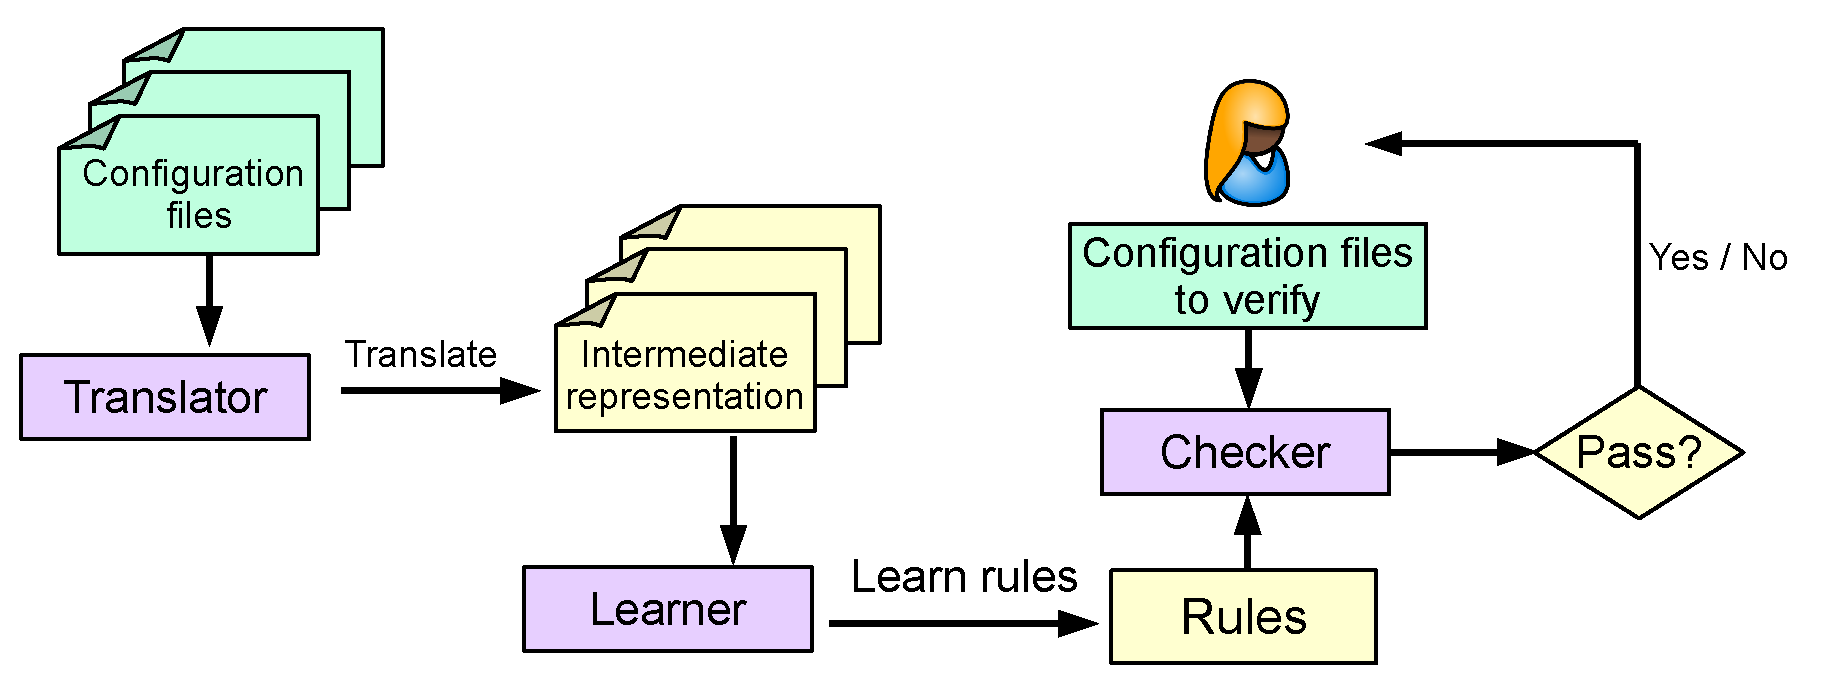
\includegraphics[width=0.78\textwidth]{figs/overview}
\caption{\app's workflow. The green boxes represent configuration files,
  including both correct general configuration files and users' input
  configuration files. The purple boxes are the components within \app.
  The yellow boxes are results generated by \app's components.}
\label{fig-overview}
\end{figure*}

We propose \app, an automatic verification framework,
which can solve configuration errors, \eg, ordering errors
and fine-grained value correlation, that previous work cannot tackle.
As depicted in Figure~\ref{fig-overview}, \app has three main steps:
translation, learning and checking. In this section, we briefly
describe how does each step work.

\para{Initial state.}
We start
with the assumption that we are given a number of (not necessarily) 
correct configuration files belonging to the same system, 
such as MySQL or Apache. 
Such files follow similar patterns, which we exploit
in a learning algorithm to build rules that
describe a language model for the files.

\para{Translator.}
The translator component first parses the input sample 
dataset (containing both configuration files and system environment
information), and then transforms them to a more structured
and typed intermediate representation.
When we run type inference on a configuration file, 
the type of a variable cannot always be fully determined from 
a single value.
We address this problem 
by introducing so called {\em probabilistic types}.
Rather than giving a variable a single type, 
we assign several types with their probability distributions. 
We can later use these more structured files
as a training set to learn the rules. 

\para{Learning.}
The learning algorithm is template-based to be easily extensible. 
We provide an initial set of templates and the
learner learns some concrete instances from the training set. These
rules are used for detecting errors violating the learned constraints
in the files given by the user.

As an illustration of a simple rule that we can learn, consider a template
 $X_1 \le X_2$, where $X_1$ and $X_2$ are
integer variables. The learner might derive the rule stating that
$\texttt{mysql.max\_persistent} \le \texttt{max\_connections}$. There is a classification and taxonomy of configuration errors in the 
existing work on automated configuration troubleshooting~\cite{yin11anempirical, configdataset}. We provide templates for every class that \app can handle: we consider integer constraints, ordering
constraints, typing constraints, and constraints about correlated entries (such as ``if $X$ is present, $Y$ has to appear as well''). 


